\documentclass[a4paper,titlepage]{article}

% Page size
%\usepackage{a4wide}

% Fonts and Language Support
\usepackage[utf8]{inputenc} 
\usepackage[T1]{fontenc}
\usepackage{mathptmx}

% Other packages
\usepackage{setspace}
\usepackage{fancyhdr}
\usepackage{fixme}
\usepackage{graphicx}
\usepackage{float}
\usepackage{listings}
\usepackage{underscore}
\usepackage{lastpage}
\usepackage{pdfpages}
\usepackage{slashbox}
\usepackage{pbox}
\usepackage[bookmarks]{hyperref}

% Macros
\newcommand{\HRule}{\rule{\linewidth}{0.5mm}}
\newcommand{\SYSNAME}{RentIt}

% Style setup
\setlength{\headheight}{15pt}
\pagestyle{fancyplain}
%\cfoot{\thepage\ of \pageref{LastPage}}
%\setstretch{1.15}

% Header and footer
\lhead{}
\rfoot{\fancyplain{}{\thepage \hspace{1pt} of \pageref{LastPage}}}
\cfoot{}

%%%%%%%%%%%%%%%%%%%%%%%%%%%%%%%%%%%%%%%%%%%%%%%%%%%%%%%%%%%%%%%%%%%%%%
% Frontpage
\begin{document}

\addcontentsline{toc}{section}{References}
\begin{thebibliography}{9}

	\bibitem{surprises}
		Judith S. Olson, Gary M. Olson\newline
		\emph{Culture surprises in Remote Software Development Teams}\newline
		ACM Queue, 2003

	\bibitem{enough}
		Niels Roesen Abildgaard\newline
		\emph{Should this be included?}\newline
		Facebook post in response to Robert Chai

	\bibitem{herbsiemens}
		James D. Herbsleb,Daniel J. Paulish, Matthew Bass\newline
		\emph{Global Software Development at Siemens: Experience from Nine Projects}
		Carnegie Mellon University School of Computer Science,
		Siemens Corporate Research 

\end{thebibliography}


% diverse
\parindent=0pt % Ingen indrykkning
\parskip=8pt plus 2pt minus 4pt

% Start on page 0
\setcounter{page}{1}

% TOC
\tableofcontents
\newpage

% Body
%\onehalfspace
\begin{spacing}{1.15}
%%%%%%%%%%%%%%%%%%%%%%%%%%%%%%%%%%%%%%%%%%%%%%%%%%%%%%%%%%%%%%%%%%%%%%

\pagebreak
\section{Introduction}

This report is written by a team of five students at the IT-University of Copenhagen (ITU)
studying Software Development on second year (4th semester).

The authors of this report are Niclas Benjamin Tollstorff (nben@itu.dk), Niels Liljedal
Christensen (nlch@itu.dk), Sigurt Bladt Dinesen (sidi@itu.dk), Kristian Brink Gansted
(kbri@itu.dk), and Niels Roesen Abildgaard (nroe@itu.dk).

The project used as a basis for this report was done in collaboration with a group of
students from the Singapore Management University (SMU), and had the goal to develop an
application that would allow users to buy and rent films and music. The application consisted
of a server developed by the ITU students and a browser-based client developed by the SMU
students.

The Singaporean team was made up of Chai Ching Hsiang Robert, Tan Kah How Kelvin, and
Chong Wen Xiong Nick.

As a part of the course \emph{System Development and Project Organisation}, we have learned
about several tools and methods to use in a software development context.

The basis for these methods is the book \emph{Project Management for Information Systems}
(5th edition) by James Cadle and Donald Yeates, which explains these methods as well
as which situations they may be used in.

We will detail project management methods used during our project, and problems that may arise
when using these. In the form of a case study, this report looks into modifications to the
methods used, and how these modifications help the project. Issues that arose during the project
are listed and paired with the methods we used to overcome them.

Finally we will analyze the effectiveness of all the methods used with an aim to determine
the usefulness of each method. The analysis is based on the team’s experiences with the
methods and is purely qualitative.

Throughout the report, we will describe and discuss our experiences with:

\begin{itemize}
    \item risk management through \emph{risk analysis}, as well as actual handling of risks
        (Sections \ref{sec:EmpiriRiskManagement} \& \ref{sec:AnalysisRiskManagement});
    \item project planning through \emph{work breakdown structure} and \emph{identification of
        dependencies}, resulting in a plan in the form of a Gantt diagram (Sections
        \ref{sec:EmpiriPlanning} \& \ref{sec:AnalysisPlanning});
    \item estimation of features through \emph{planning poker} (Sections
        \ref{sec:EmpiriEstimation} \& \ref{sec:AnalysisEstimation});
    \item choice of development framework (or methodology) for a small project (Sections
        \ref{sec:EmpiriOrganizational} \& \ref{sec:AnalysisOrganizational});
    \item quality control, using a \emph{quality plan} (Sections \ref{sec:EmpiriQualityControl}
        \& \ref{sec:AnalysisQualityControl}); and
    \item progress monitoring, keeping in mind the initial planning and estimation (Sections
        \ref{sec:EmpiriProgress} \& \ref{sec:AnalysisProgress}).
\end{itemize}
\pagebreak

\part{Empirical Evidence}
\label{chap:Empiri}
In this part we will describe the methods from Cadle and Yeates\cite{caye} used in the project, how we used them, and any issues we may have experienced with them.

The aim is to give a look in to how every method works and how we chose to adapt it to our specific project. This will be the basis of the analysis in part \ref{chap:Analysis}.

\section{Risk Management}


\addcontentsline{toc}{section}{References}
\begin{thebibliography}{9}

	\bibitem{surprises}
		Judith S. Olson, Gary M. Olson\newline
		\emph{Culture surprises in Remote Software Development Teams}\newline
		ACM Queue, 2003

	\bibitem{enough}
		Niels Roesen Abildgaard\newline
		\emph{Should this be included?}\newline
		Facebook post in response to Robert Chai

	\bibitem{herbsiemens}
		James D. Herbsleb,Daniel J. Paulish, Matthew Bass\newline
		\emph{Global Software Development at Siemens: Experience from Nine Projects}
		Carnegie Mellon University School of Computer Science,
		Siemens Corporate Research 

\end{thebibliography}

\section{Estimation}
\label{sec:EmpiriEstimation}

We used a number of estimation methods introduced in the book \cite[ch.~9]{caye} and throughout the
course. This section attempts to explain these as well as the rationale behind our choices.

Once we had identified the activities in our project, with the work breakdown structure method,
estimates as to how long time the activities would take to complete could be made. In our project
and team we faced several challenges with regards to estimating accurately.

\begin{itemize}
\item The five of us had never worked together on a project before, which made it hard to factor
    in how time consuming communcation and teamwork in general would be. We had no previous experience
    or metrics to base our estimates on.
    
\item Part of the project was done by Singaporean students who we had not even met when we did the
    initial estimates. Not knowing how much experience they had in similar projects and with the web
    service technologies was a major complication in estimating.
    
\item We were working with technologies that were new to us. This made it hard to estimate activities
    involving these new technologies as we did not yet know how complicated they would be.
\end{itemize}

\subsection{Direct estimation}

As the work breakdown structure was already done, the natural choice for us was to use the \emph{direct
estimation method}\cite{caye}. The method bases its estimation on the activities discovered by the work
breakdown structure or project breakdown structure method. Each activity is  estimated separately, by
one or more qualified estimators. Eventually all of the activity estimates add up to the total project
estimate. 

For the estimation of the individual tasks we used a method called \emph{planning poker}, which is commonly
used in Scrum teams. In the method each team member has five pieces of cardboard with \textbf{small},
\textbf{medium}, \textbf{big}, \textbf{too small}, or \textbf{too big} written on them. Each task is
introduced and every member selects the piece of cardboard they believe to best describe the size of the task.
The people with the highest and the lowest estimate then explain their views on the task. After that the
process is repeated until all group members agree on an estimate. The final estimates were the basis for our
dependency diagram (Appendix \ref{app:dependencydiagram}).

We chose this method to ensure that everyone in the group got their say and because it seemed to work well in
the Scrum methodology as having estimates for all tasks is key in sprint planning (see Section
\ref{sec:EmpiriOrganizational} for an explanation of sprints as well as our general use of Scrum). To further
facilitate easy sprint planning we decided to estimate testing of tasks separately from the task itself, this
should also lead to better estimates in the future as it will create better metrics to reference.
\section{Organizational framework and development approach}
\label{sec:organizational}

As a team we have no say in what kind of organization we are in – it has been pre-decided. Our
situation can be seen as a \emph{pure} project organization\cite{caye}, where individual project members are
pulled from several departments to focus on a project. In our case these departments are the
ITU and the SMU.

There are, however, other concerns to be had. None of the team members are working exclusively
on this project (due to other concurrent courses at their respective universities) and meeting
times can vary a great deal.

%NOTICE CITATION NEEDED

Using a software development methodology (used here as a catch-all term for approaches to
development, often consisting of several \emph{methods} or \emph{practices}\footnote{In other
words, using the definition found on Wikipedia: "A \textbf{software development methodology}
or \textbf{system development methodology} in software engineering is a framework that is used
to structure, plan, and control the process of developing an information system."
http://en.wikipedia.org/wiki/Software_development_methodology}) for a project can help to
improve quality of the product, as well as decrease the frequency of various issues \textbf{
(citation needed lol)}. Different methodologies have different focuses and, as a result of
this, mitigate different kinds of issues. Methodologies come in many shapes and sizes, and we
considered several of these before deciding on using Scrum internally in the Danish team.

Scrum uses an iterative approach (as opposed to a linear approach), where certain steps are
repeated rapidly and continuously to bring in more functionality step by step (instead of
introducing it all at once).

When using Scrum, there is less bureaucracy required\cite{caye} which allows us to quickly set up a project
group and get started. As the project is rather small in scope, it seems ideal to avoid any overhead
that is not strictly required.

Usually, a project would be split into 30-day sprints when using Scrum; however, due to the size of
our team and project, we chose to work with 7-day sprints instead. A sprint is a period in which the
team focuses on a pre-determined set of features. The set of features is explained as stories,
explaining how a user would interact with the application.

On meetings between each sprint, a \emph{backlog} for the entire project is maintained (more stories are
added, obsolete stories are discarded, stories with changing requirements are edited) and the stories
for each sprint are picked from this prioritized pool. The set of stories for a single sprint is known
as the \emph{sprint backlog}.

In a Scrum team there is a Scrum Master who ensures that all members of the teams follow the guidelines
of the methodology. This includes standing up at daily meetings (which we chose to have on a weekly basis),
maintaining the various backlogs, and more.

In our case, the Scrum Master had to take on multiple roles and also work as a developer, as we are a relatively
small team that would not have been effective otherwise (losing 20\% of our workforce).

While using scrum, we faced several issues.

Because of the volatile schedules of each team member, it was often hard to find days to meet and work
together. We ended up having just part of a single day every week, often meeting up in pairs or working
from home.

There were several factors resulting in some weeks having very active development and others being almost
completely stagnant (no work done). This had a lot to do with schedules of other courses colliding in
time-consuming ways.

It was hard to maintain a Scrum Master role from afar because it is a role that requires observing the
team. Keeping in touch through online communication did make this possible, although it was far from a perfect
solution.

\section{Project Control}
\label{sec:EmpiriControl}
This section attempts to explain how we secured the quality of our project, as well as how we kept control of tasks, making sure that everything we set out to do was actually done.

\subsection{Quality Plan}
\label{sec:EmpiriQualityControl}
To ensure that our project kept a certain standard, we made a simple quality plan\cite[ch.~14.4.2]{caye} to describe what is considered good quality and how we should test the quality.

In order for a piece of the program to be accepted as having high enough quality, we
agreed that it must:

\begin{itemize}
    \item use responsible error handling;
    \item be well documented and readable by peers of the author;
    \item be tested with all inputs (equivalence groups); and
    \item fit in the API described in the design.
\end{itemize}

To check that the program lives up to the quality requirements, all tasks must go through a peer review before being accepted as done. The program will then have to be tested systematically to assure it upholds the quality requirements. If the program passes these tests, it is considered done and can be delivered.

The responsibility of the quality of a delivered piece of program lies with the author
and the reviewer. The reviewer should also review the tests made for the program and
the results of these tests. If the delivered program does not live up to the quality
requirements, both will be held responsible.

\subsection{Monitoring Progress}
\label{sec:EmpiriProgress}

Monitoring the progress of a project helps to determine if the deadlines can be upheld.
If this is not the case, it is important that this is discovered as soon as possible,
allowing new and more precise estimates to be made, and more realistic deadlines.

Our progress monitoring was based on two vital artifacts: the Scrum backlog and the network
diagram with critical path. The backlog is a very strong tool for monitoring the progress
of projects as it allows a project manager to easily get an overview of the current state
of the project.

With the sprint backlogs, the manager can see the progress of the individual tasks to zero 
in on what task exactly is lacking behind. Based on the backlogs we were also able to create 
burndown charts (can be seen in appendix \ref{app:burn}). These helped increase the ease 
with which the manager could get an overview of the projects and the individual sprints' progress. 
The burndown charts were available to all group members which allowed everyone to follow the progress.

The network diagram with its critical path is a good supplement to the backlogs because it
makes it easy to tell which activities should be prioritised if the manager needs to save
some time. Combined, these two artifacts function like the conventional time sheet as
described by Cadle \& Yeates\cite[ch.~11]{caye}.

\pagebreak

\part{Analysis of Methods}
\label{chap:Analysis}
In this part we will discuss the results of using the methods described in Part \ref{chap:Empiri}, focusing on which uses were and were not successful and potential improvements.

\section{Analysis of Risk Management}
This section takes a look at how our risk management went, including thoughts on what went well and what could have been done differently.
\label{sec:AnalysisRiskManagement}

There are two areas of concern when analyzing the effectiveness of risk
management:

\begin{enumerate}
\item The issues or difficulties we avoided by doing a risk analysis early on,
and what issues we did not predict, but still ended up facing. Looking
at these will give us an idea of how much we gain from using a risk analysis.
This is based mostly on qualified guesses.

\item Issues when performing the analysis itself, and how much effort
it requires to complete such an analysis.
\end{enumerate}

These two areas together give us an idea about whether the \emph{benefits} of the risk analysis are
ultimately worth the \emph{effort} required.

\subsection{Effectiveness of Preventive Analysis}

In the empirical section we highlighted three different risks to be focused on and handled. These risks
will be the focus for determining the effectiveness of our risk analysis.

We place each of the risks considered in one of the categories \textbf{very effective}, \textbf{some
effect}, and \textbf{no effect}, to facilitate further discussion.

\subsubsection{P2: Project overhead}

Because we realized early on that project overhead was an issue, we planned around this and succesfully
avoided this risk entirely. Our team worked in a highly agile fashion, and the choice of methodology helped
us stay on target.

Avoiding this risk proved \textbf{very effective}.

\subsubsection{Req1: Requirements are changeable}

Discussing requirements and common interfaces requires involvement of several
parties. We had several discussions with the Singaporean team, that led to a
firm belief that our contact surfaces were going to stay more or less the same.

As it turns out, either due to bad communication or misunderstanding of
expectations, the Singaporeans did not see these early discussions as anything
close to final.

During the final week of collaboration a lot of requests for changes to the
common interfaces surfaced, putting a heavy load on the Danish team and
requiring some minor changes to the internal data structure.

The mitigation of the risk was not entirely successful, and this shows that no
matter much is done to mitigate or avoid a risk, it is impossible to be entirely
safe.

The mitigation did, however, make sure the most central interfaces (and hence
most of the internal data structure) could be preserved. The initial discussions
did have \textbf{some effect}, however not as much as desired.

\subsubsection{T4: Development differs from Live}

The final risk we chose to focus on had to be accepted, because we were unable to do
anything to handle it before starting the project. Having done the analysis, however, was a great help
as it made us aware of this potential threat to development stability.

Because of this awareness we focused on getting the live and development environments as synchronized as
possible as well as developing a clear protocol for updating configuration files for the servers, in
order to avoid any discrepancy.

Had we not had these protocols in mind it is very likely that this could have developed into a serious
roadblock for development. Although any such risk is entirely hypothetical (as we have not tried this
situation without first doing a risk analysis) it seems fair to assume that it was a nice safe-guard to
have in place.

Spending time on this risk had \textbf{some effect}.

\subsubsection{Unavoided risks}

Because the risks were prioritized and only the first few handled, some risks
could come up as issues and hit development with full force. One such case was a
risk that we had actually anticipated, but chosen not to handle: the fact that
we were developing a new type of application (\textbf{Risk T2}).

Unknown technology may be more complex than first anticipated, and this proved
to be true for our situation. We had only anticipated a few possible issues,
but had not anticipated the one that hit us.

As it turns out it was difficult to send out responses with the proper HTTP
error codes when using an IIS based WCF service. As this was not exactly
blocking further development, the impact was limited, but it was an issue that
took a substantial amount of time to fix.

Turns out we never actually wore pants.

\subsection{Effort Required}

Our risk analysis was performed as a group discussion, where any and all concerns were brought up to scrutiny.
As it turns out, with a project of the size we undertook, the number of concerns was limited. After an initial
discussion we had a couple of days to come up with any additional risks or revisions and then a final discussion
to implement these.

All in all the effort required was rather small, and the planning was done in a matter of hours. Efforts to actually
mitigate or avoid risks were more substantial, but could mostly be seen as development time. This time was kept
negligible by choosing to only focus on a few risks. This could have been adjusted by trying to avoid or mitigate
additional risks.

\subsection{Cost vs Benefit}

With the amount of effort we put into the analysis (cost) and the effect it yielded (benefit), there can be no doubt
that this practice of analyzing risks is very recommendable, with some to high effectivity and little effort (the
benefit is worth the cost).

In a situation with as few potential risks as ours it would be recommendable to attempt avoiding or mitigating more
risks than we did in our particular situation. We were hit by a risk that was placed in the second-highest category,
moderate impact, medium likelihood. If we had chosen to handle the risk in this category a great challenge may have
had less of an impact.

\section{Analysis of the Planning Process}
\label{sec:AnalysisPlanning}

This section explains our thoughts on the different tools used in planning our
project, as well as how useful they were.

\subsection{Work breakdown structure} In an attempt to discover and organize
the work in front of us, a work breakdown structure was created. It created a
rhetorical turmoil as the diagram itself, rather than the structure it
abstracts, became subject of our focus and conversation.

At the time, we were not yet entirely clear on what work would need to be done,
and so the diagram was shallow and vague. Our situation left us especially
prone to discussion as the problem domain was rather new for us, making it
difficult to conclude on what needed to be done. In retrospect, a product
breakdown structure may have been the appropriate tool at the time. Making a
tree of products rather than activities would have allowed us to focus on
\emph{what} needed to be produced, and delay making decisions on \emph{how} to
produce it\cite[ch.~8.3,~8.4]{caye}.

\subsection{Activity dependencies}
Something that \emph{did} work out for us was the identification and
satisfaction of dependencies. Our initial time estimates were imprecise, but
still gave us the advantage of knowing the order in which to approach
activities. While seemingly trivial, failure to assert activity dependencies
could have caused much frustration and wasted a lot of time. Having previously
learned this the hard way in previous projects, there was little inclination to
discuss the validity of dependency analysis.

While network diagramming is a fairly rich and explicit representation of
inter-activity dependencies, they are not easy to read. Gantt
diagrams, on the other hand, are easy to read, perhaps because they are more
abstract. Gantt charts do not describe things such as slack and the critical
path, but provide a less information-cluttered overview. As such, Gantt charts
may not be very helpful in the planning process, but are useful for describing
and quickly getting an idea of the plan itself.

Gantt diagrams can show much more than just activities over time, and can quickly
get cluttered\cite[ch.~8.6]{caye}. We chose to show dependencies, but other than
that stuck to the most basic formula. In practice, whenever we needed to
check inter-activity dependencies, we ended up consulting the network diagram
instead, as it was more detailed. Therefore, there was no real need to include
dependencies in the Gantt chart.

While not bulletproof, this kind of planning can decide success or
demise\cite[ch.~8]{caye}, especially for larger projects, where the risk of
losing the overview is increased. The bigger picture painted by the use of
these tools can uncover hidden issues, and help prepare for more obvious ones.

\section{Analysis of Estimation Methods}
\label{sec:AnalysisEstimation}
\subsection{How did it go?}
Planning poker allows every member of the group to give their initial estimate of a task uninfluenced by the estimates given by the rest of the group, because everyone reveals their estimate at the same time. This gives everyone the chance to explain their estimate, perhaps making other group members realize that their initial estimate was wrong, which was the case during several of our SCRUM meetings. It also invites discussions of the different tasks to be estimated which can help to clarify what the task in question is about (people may reach different estimates because they have understood the tasks differently), which is a definite quality we found in using this estimation method. While time consuming, we feel that using planning poker has definitely paid off, both in terms of estimating and in terms of understanding and defining our tasks.

\subsection{Alternative Estimation Methods}
Seeing how well the planning poker method worked, the Delphi technique \cite{caye} might also have been useful as it follows the same idea of letting people change their estimates depending on estimates given by the rest of the group. However, with the Delphi technique being anonymous in the sense that each estimator gives their estimate anonymously, estimators will not be given the chance to explain why they have estimated a given task they way they did. Being anonymous, though, it allows estimators to be less concerned about changing their estimate to comply with the rest of the group if they are certain their estimate is the right one. In some ways this method might be better than the planning poker method because of its anonymity, but being anonymous might also make it less ideal in some circumstances (for example, if two estimators disagree and both refuse to change their estimates).

Another estimation method that might be suitable is the Analysis Effort method \cite{caye} in which the team estimates the effort needed for the analysis part of each individual program function. Then, by considering a series of factors such as team size, familiarity with the type of work, and complexity, the ratio between analysis, which has now been estimated, and design, coding, and testing. In total, this gives an estimates of the entire project and subtasks of which it is composed. This is a somewhat stricter estimation method than planning poker and the Delphi technique as the factors are less up to interpretation than simply giving a number to represent an estimate. For example, if the team size is known, this factor will always be the same. Leaving less to imagination and interpretation of the factors used to determine the estimate could be useful in groups that are less experienced in estimates (like our own) as there is a template to follow.
\section{Analysis of Development Process}

Scrum is a widely used and very popular software development methodology. This shows in the amount
of articles found about it online and discussions about how to use (or even improve) it. This means
that there are many different versions of Scrum based on different company and team profiles. They
all inherit the same structure, but some numbers vary.

One thing that has changed for Scrum is the length of sprints. The traditionally recommended 30-day
sprints have been replaced by a guideline that says that each iteration should be "no more than four
weeks each (the most common is two weeks)"\cite{scrumprime}.

Seeing as we are a very small team working on a relatively small project, it seems natural to have as 
short iterations as possible: The shorter the iteration, the more \emph{agile} we get - we are quicker
to adapt to changing situations. With a total project length of less than three months it would be
dangerous to lock in backlogs 30 days at a time.

We opted for more iterations of a shorter duration and landed on a week as a well-fitting size. This
proved a great help as we had many changes to requirements, sometimes several in the same week. Because
we could rapidly adjust our course this had little impact on our work.

\subsection{Stand Up Meetings}

In our weekly meetings, where we would follow up on what had been done as well as discuss what would be
next, we didn't always actually \emph{stand up}. The meetings were fairly rare, but a great way of
motivating the team. If it had in any way been possible to have these meetings more than weekly this would
likely have added to our productivity. Unfortunately this wasn't possible due to our schedules.

At the meetings where we were standing we noticed an increase in pace, focus and motivation: all team members
were more eager to get started with the day's work, and do it well. A heightened focus on standing would
likely have had a positive effect.

\subsection{Stagnant sprints}

Sprints in which no work was done were a real problem in the project. We did not fall behind schedule because
of these, but it did make development highly irregular, resulting in more meetings where all team members
would be brought back up to speed.

Additionally when only working in spurts, these spurts were much more intense. Some sprints were stagnant, but
others required long work days, resulting in a decline in our productivity\footnote{This is a well-known issue
that is covered in Kent Beck's \emph{Extreme Programming Explained}\cite{xpe} as well as in other fields of
research\cite{workingtime}.}.

To avoid stagnant sprints, we could have made a schedule over how many hours each member could work each week
and make sure that some work was done each week. This would have solved most of our problems in this area. It
would immediately reduce work in active sprints, and lessen time spent in meetings.

On the other hand most factors that added up to stagnation were unpredictable and out of our hands so the effect
of creating such a schedule is dubious. Having a schedule is one thing, sticking to it is another. With several
concurrent projects for each team member it is hard to have a regular schedule.

\subsection{Final words}

All in all, using Scrum helped us avoid a serious risk for the development timeframe\ref{sec:RiskManagement} as
well as provide a general framework.

We made some helpful changes to the process, but did not enforce some important parts of the methodology, which
would have been helpful had they been enforced.
\section{Analysis of Quality Plan}
\subsection{Jeg kan ikke finde på titler!}
Having a quality plan has made it easy for us to check whether a certain part of the program meets our quality standards. Since it is the same routine for every part of the program, it has proven, in time, to get easier and quicker to do a quality check. Agreeing on what we define as quality also makes it easier for each individual group member to trust that, once a part of the program has gone through quality checking, it is of quality, even if the quality check was done by another group member entirely (gief omformulering?).
\pagebreak
\section{Conclusion}
(be subjective (we have) or objective (it has)?) Several of the methods and tools presented in the book \cite{caye} were found to be useful in a project like this one, while others were not (passer det? :P). 
An estimation method as simple as Planning Poker has proven to be were useful due its ease of use, needing almost no introduction, as well as its proneness to start discussions about the tasks being estimated, all without taking very much time to perform.
The use of a quality plan has reduced the time needed to perform quality checks on program parts, freeing up more time to do actual work.
One tool that has proven to be a very useful tool in software development is Scrum because it allows the project to evolve and change over time, thus also allowing the requirements of the product to change. Its agile nature makes it work well with a lot of estimation methods because it allows for tasks to be estimated anew, multiple times, should the previous estimate have been too ambitious. The flexibility of Scrum allows a project group to tailor it to their needs. Being able to run short sprints has been an absolute necessity as the Singaporean team had a lot of spontaneous requirements that needed to be accommodated and incorporated into the requirements as soon as possible.

Mere?
\section{Reflection}

We have found that in small projects like this, one of the most important
things is to be able to see the project progress at all times. The Scrum
backlogs are a really intuitive way of monitoring the progress of a project and
it works really well with small projects, so that is definitely something we
would recommend using in situations similar to ours.

To make the backlogs useful it is very important that the estimates produced
are accurate. We learned that this is a hard thing to do well and it is a fine
balance between time spent estimating and the needed accuracy of the estimates.
The use of a work breakdown structure followed by planning poker worked well for
us, but it is quite time consuming, the task growing exponentially with the
size of the project, and therefore we would only recommend it in smaller
projects.

In general we were really happy with working with Scrum, it seems like a really
solid organizational framework which works very well inl projects like this. We
can recommend if for all smaller projects in which an iterative approach can be
used. 


% section problemstatement (end)
%%%%%%%%%%%%%%%%%%%%%%%%%%%%%%%%%%%%%%%%%%%%%%%%%%%%%%%%%%%%%%%%%%%%%%
\end{spacing}
%%%%%%%%%%%%%%%%%%%%%%%%%%%%%%%%%%%%%%%%%%%%%%%%%%%%%%%%%%%%%%%%%%%%%%
%Bibliography
%\addcontentsline{toc}{section}{References}
\pagebreak
\addcontentsline{toc}{section}{References}
\begin{thebibliography}{9}

	\bibitem{surprises}
		Judith S. Olson, Gary M. Olson\newline
		\emph{Culture surprises in Remote Software Development Teams}\newline
		ACM Queue, 2003

	\bibitem{enough}
		Niels Roesen Abildgaard\newline
		\emph{Should this be included?}\newline
		Facebook post in response to Robert Chai

	\bibitem{herbsiemens}
		James D. Herbsleb,Daniel J. Paulish, Matthew Bass\newline
		\emph{Global Software Development at Siemens: Experience from Nine Projects}
		Carnegie Mellon University School of Computer Science,
		Siemens Corporate Research 

\end{thebibliography}


%%%%%%%%%%%%%%%%%%%%%%%%%%%%%%%%%%%%%%%%%%%%%%%%%%%%%%%%%%%%%%%%%%%%%%
% Appendices
\newpage
\appendix
\part*{Appendices}
\addcontentsline{toc}{part}{Appendices}
\section{Risks}
\label{app:risks-appendix}

\subsection{Technical Risks}
\begin{description}
    \item[T1 New development environment] In the project we will be working with an unfamiliar
        framework (.NET’s WCF) and server technology (IIS). If any problems arise with these
        technologies they will considerably lengthen the project scope as no member of the team
        would have the required familiarity to quickly solve such a problem. On the other hand
        it is not very likely that any problems should arise as WCF is used through C\#, a
        programming language the entire team is familiar with, and the interface to the IIS-server
        is very much like using Windows on a desktop computer.\newline
        \textbf{\emph{Impact: moderate; Likelihood: low}}
    \item[T2 New type of application] None of the developers have previously developed a WCF-based
        RESTful service. This technology will require some self-education on various points. It is
        fairly likely that the team would end up in situations with lack of knowledge, and this may
        take a considerable amount of time to get around.\newline
        \textbf{\emph{Impact: moderate; Likelihood: medium}}
    \item[T3 New language] Few of the developers have ever worked with the JavaScript Object Notation,
        which will be a vital part of the service built. The syntax, however, is very simple and easy
        to learn, so it seems unlikely that this would amount to an actual problem.\newline
        \textbf{\emph{Impact: small; Likelihood: low}}
    \item[T4 Development environment differs from Live environment] The environment present on
        developers' computers as well as the way WCF applications are tested locally, differs vastly
        from the way the code is deployed. This requires the maintenance of two different (but similar)
        configuration files. It is likely that there will, at some point during the project, arise a
        situation where there is some inconsistency between the two, resulting in improper tests. This
        could be everything from very easy to very hard to fix, depending on the situation.\newline
        \textbf{\emph{Impact: moderate; Likelihood: high}}
\end{description}

\subsection{Planning and resource risks}
\begin{description}
    \item[P1 Time constraints may be exceeded due to scope of project] The size of the project may have
        been underestimated, and the project may require more man-hours than originally planned. Due to the
        actual (small) scope of the project this is not likely, and if it did happen it is likely that the
        team members would be able to move around their schedule to put in more work, so the impact would
        not be high.\newline
        \textbf{\emph{Impact: small; Likelihood: low}}
    \item[P2 Time constraints may be exceeded due to project overhead] Starting a project, especially when
        it is a small one, requires a relatively large amount of overhead (bureaucracy, preparation). This
        often requires for the entire team to assemble and agree on the terms by which they work.\newline
        \textbf{\emph{Impact: moderate; Likelihood: high}}
\end{description}

\subsection{Requirement risks}
\begin{description}
    \item[Req1 Requirements are changeable] As the requirements are a product of two teams (separated by
        space, and often time) discussing their wants and needs, it is very likely that they will be very
        volatile. Changing requirements early on is not a problem, but the later they change the more of an
        impact they will have on the development, as more of the product will have to be scrapped and redone.
        \newline
        \textbf{\emph{Impact: moderate; Likelihood: high}}
    \item[Req2 Requirements lack detail or are ambiguous] When discussing requirements the final version may
        be subject to some ambiguity, often the result of earlier misunderstandings. This may result in one
        team implementing a feature that will not work with what the other team has implemented. It is fairly
        likely that such a discrepancy will develop during global software development, but as the overall
        idea will most likely be preserved it is unlikely that fixing such an issue will amount to very much work.
        \newline
        \textbf{\emph{Impact: small; Likelihood: medium}}
\end{description}

\section{Gantt chart of plan}
\label{app:gantt}
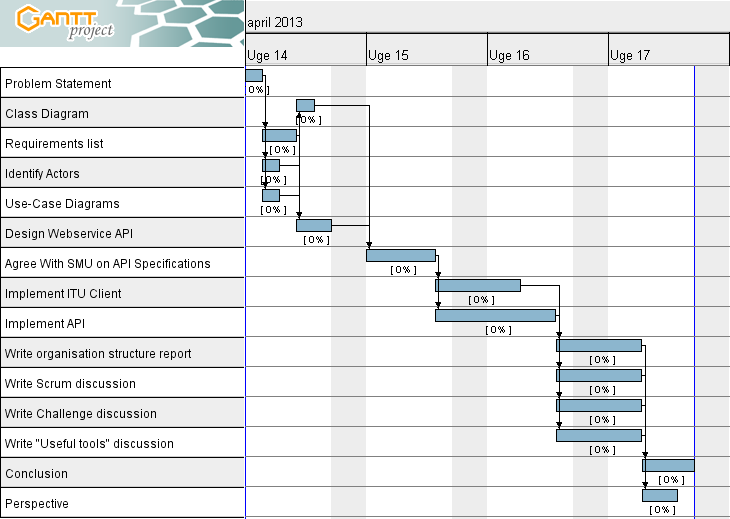
\includegraphics[scale=0.5]{./Empiri/Planning/img/gantt-chart.png}
\emph{Gantt chart with dependencies (grey lines), critical path (activities
in red), and milestones (yellow)}

\section{Dependency Diagram}
\label{app:dependencydiagram}

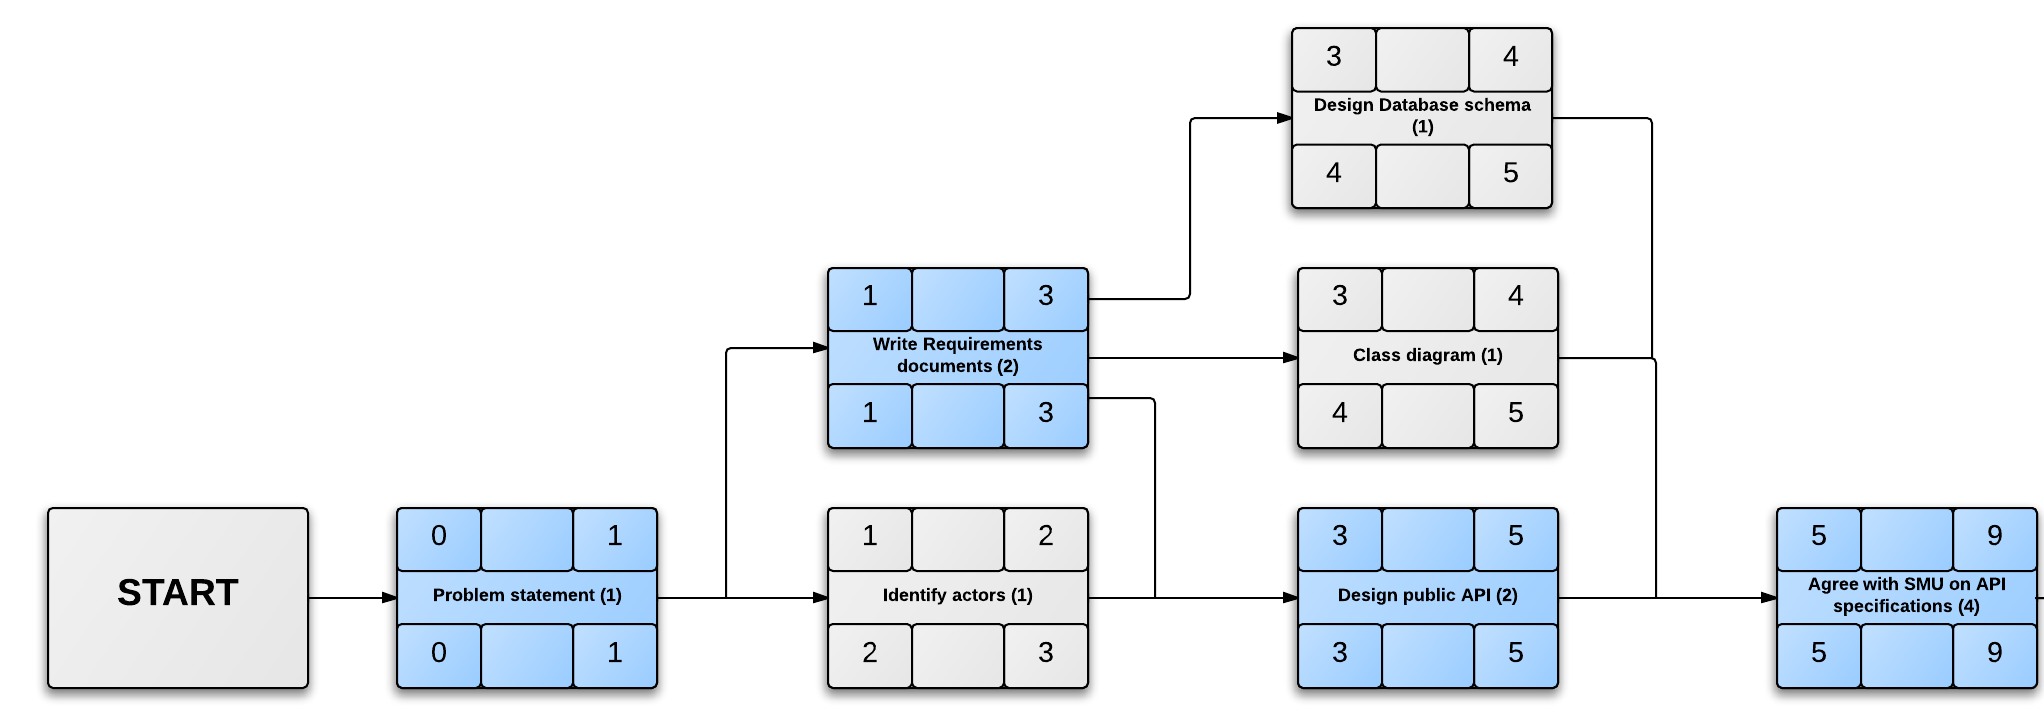
\includegraphics[scale=0.2]{./Appendices/networkdiag-p1.png}

(notice that the diagram wraps around and continues below)

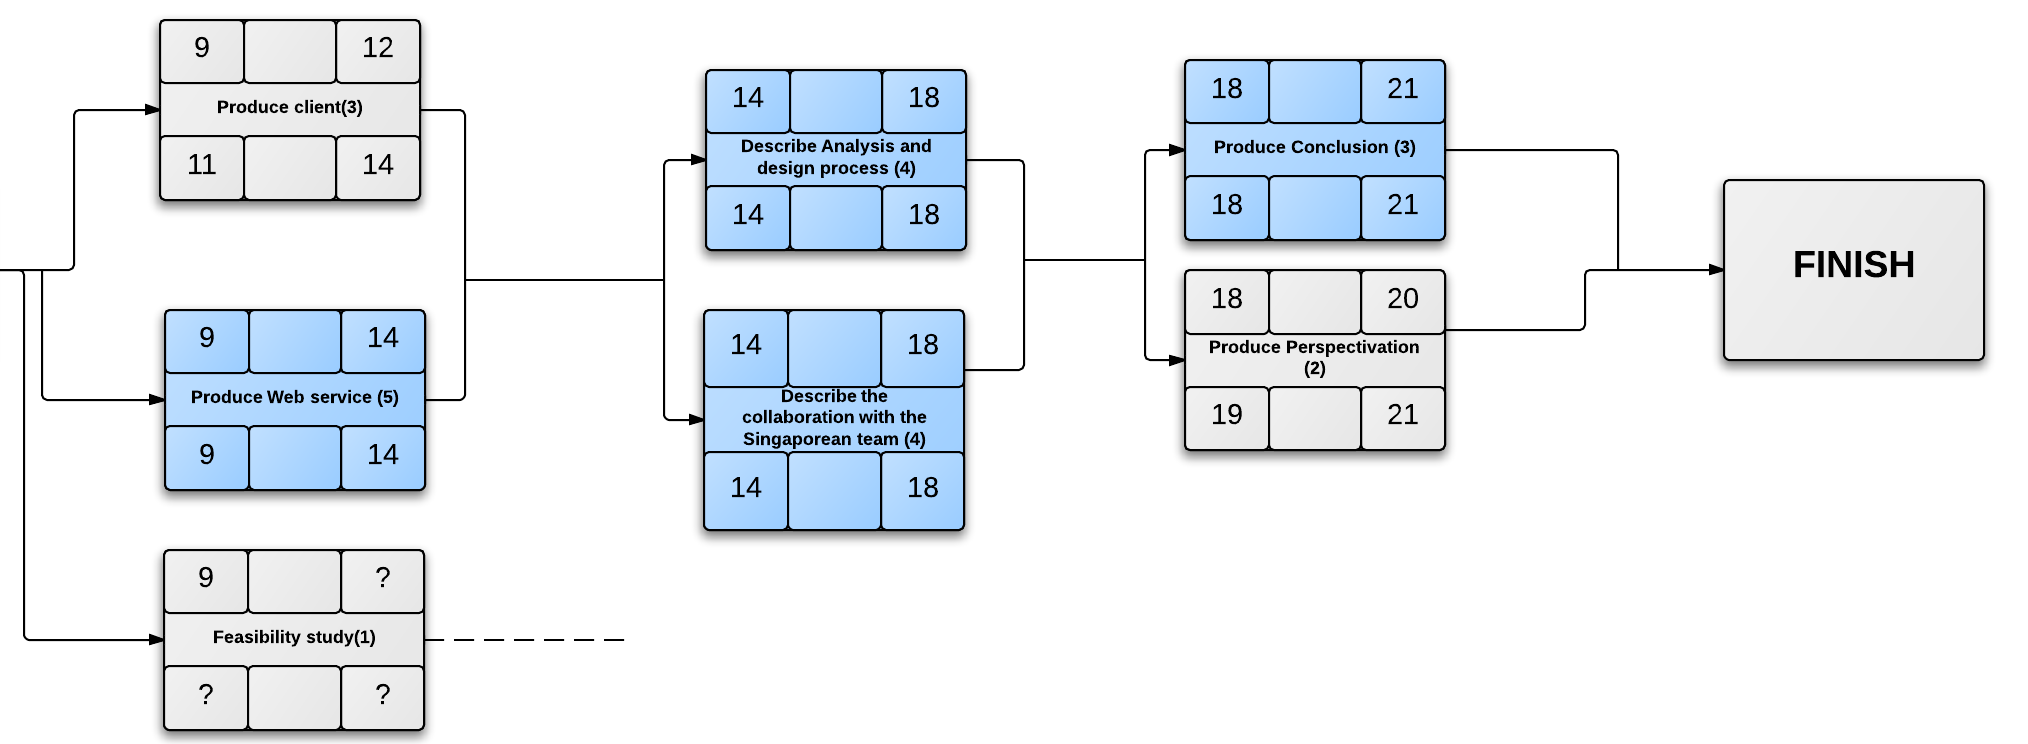
\includegraphics[scale=0.2]{./Appendices/networkdiag-p2.png}
\section{Milestones}
\label{app:milestones}
Milestone 1:
\begin{itemize}
\item To be done: Initial problem statement
\item Approval criteria: Agreed upon by all group members
\item Approval method: Dialogue
\item Approved by: All group members
\end{itemize}

Milestone 2:
\begin{itemize}
\item To be done: Requirements specification
\item Approval criteria: External approval from SMU group
\item Approval method: Revision
\item Approved by: SMU group
\end{itemize}

Milestone 3:
\begin{itemize}
\item To be done: Webservice API and datastructure
\item Approval criteria: Agreed upon with the SMU group
\item Approval method: Dialogue
\item Approved by: All group members and the SMU group
\end{itemize}

Milestone 4:
\begin{itemize}
\item To be done: Implementation of webservice and ITU client 
\item Approval criteria: Must uphold requirements and API agreement
\item Approval method: Systematic testing, and revision
\item Approved by: All group members
\end{itemize}

Milestone 5:
\begin{itemize}
\item To be done: Main parts of the report 
\item Approval criteria: The discussions of the report are done and approved upon by all group members
\item Approval method: Dialogue
\item Approved by: All group members
\end{itemize}

Milestone 6:
\begin{itemize}
\item To be done: Report
\item Approval criteria: No grammatical errors and all content is outstanding
\item Approval method: Proofreading
\item Approved by: All group members and GOD
\end{itemize}

\section{Work Breakdown Structure}
\label{app:workbreak}

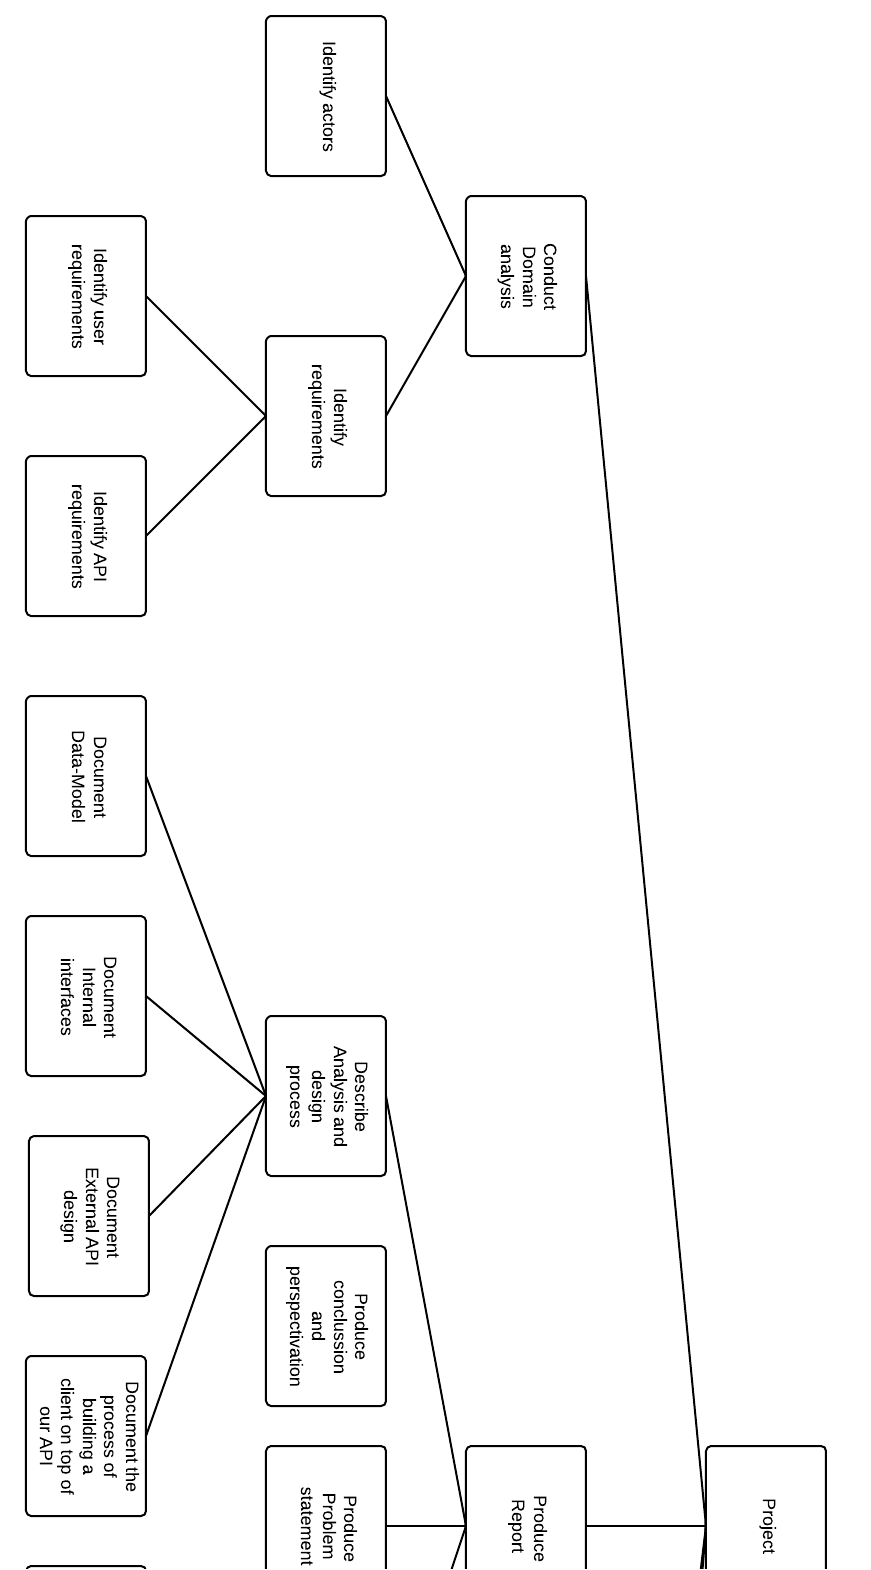
\includegraphics[scale=0.45]{./Appendices/workbreakdown-p1.png}

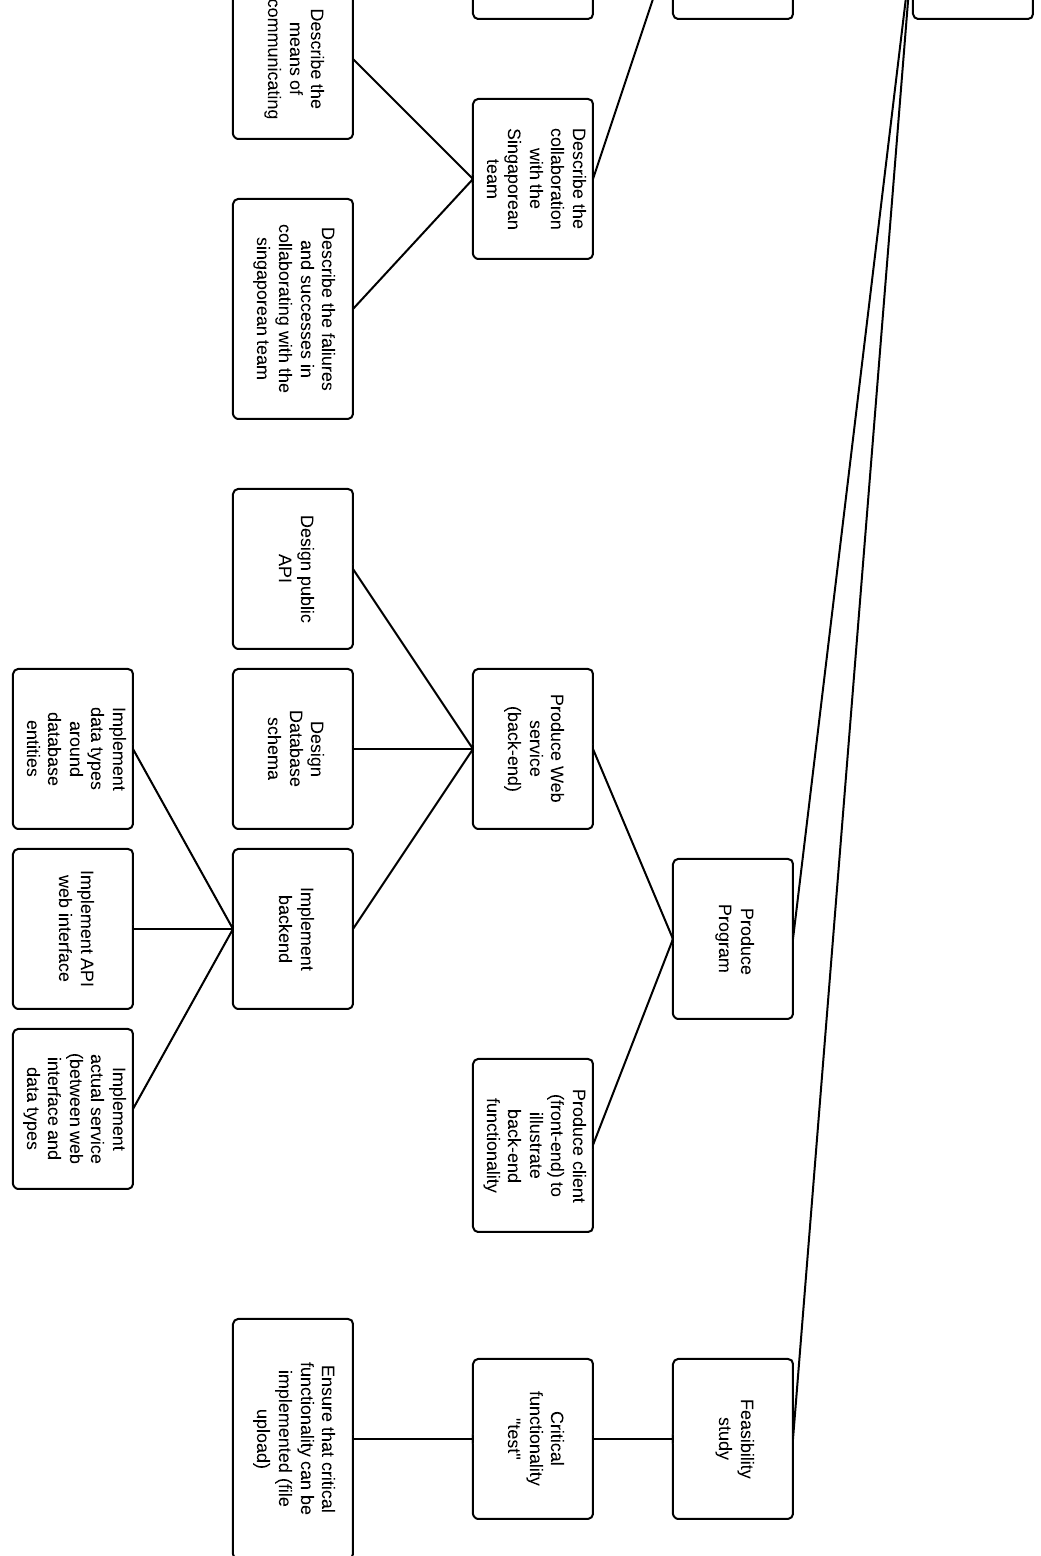
\includegraphics[scale=0.46]{./Appendices/workbreakdown-p2.png}
\addcontentsline{toc}{section}{Burndown Charts}
\label{app:burn}

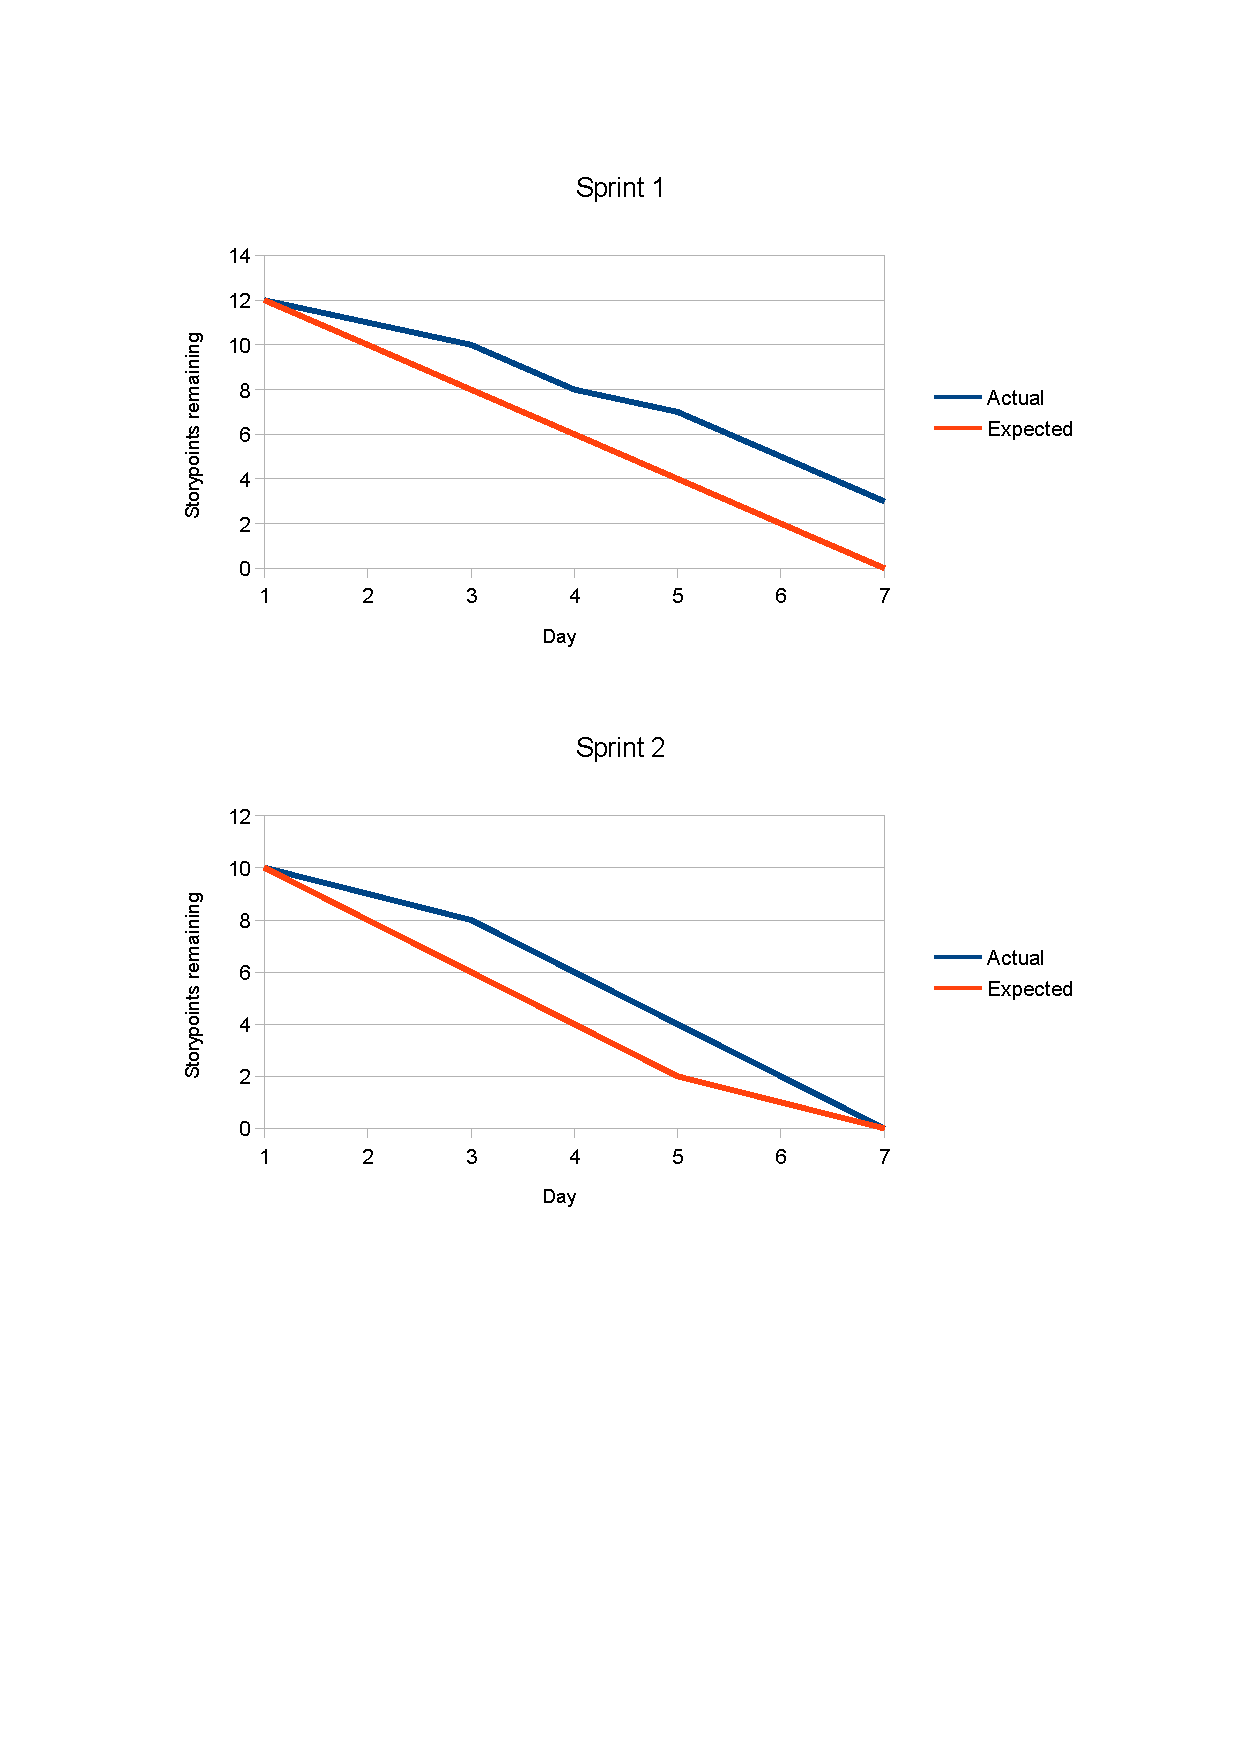
\includepdf[pages={1-3}]{./Appendices/burn.pdf}


%example appendixsect
%\section{Deployment View} % (fold)
%\label{app:deployment}
%\includegraphics[scale=0.7]{figures/DeploymentView.jpg}
%
%% section deployment (end)

\end{document}
